\documentclass[a4paper,12pt]{book}
\usepackage[spanish]{babel}
\usepackage[utf8]{inputenc}
\usepackage{graphicx}
\usepackage{titling}
\usepackage{makeidx} % Paquete para el índice
\usepackage{fontspec}
\usepackage{tabularx}
\usepackage[acronym,nonumberlist,nopostdot]{glossaries}
\usepackage{subfig}
\usepackage{caption}
\usepackage{url}
\usepackage{apacite}
\usepackage{lipsum}
%\setmainfont{Noto Sans CJK KR}
\usepackage{CJKutf8}
\usepackage{kotex}



\title{Hwarangdo\textregistered: El Camino de los Hombres Florecientes}
\author{Guillermo Rojas}
\date{\today}

\makeindex % Inicializar el índice

\makenoidxglossaries
\input{glosario.tex}

\begin{document}

	\begin{titlepage}
		% Añadir un término al glosario

		\centering
		\vspace*{\fill}
		
\includegraphics[width=0.7\textwidth]{images/sam_taeguk.png} % Reemplaza 'Hwarangdo\textregistered_logo' con el nombre de tu archivo de logotipo
		\vspace*{\fill}

		\vspace*{2cm}

		{\Huge\bfseries Hwarangdo\textregistered: El Camino de los Hombres Flores\par}
		\vspace{2cm}
		{\Large Tú Nombre\par}

		\vspace*{\fill}
		{\large \today\par}
	\end{titlepage}

	\tableofcontents
	% Índice generado automáticamente|

	\frontmatter % Cambia al estilo de numeración de páginas romanos para las partes iniciales

	%	El archivo entre {} debe ser \invlude{/ruta/al/nombredelarchivo} y el archivo tiene que tener .tex


	\chapter*{Agradecimientos}

En esta sección, puedes expresar tu gratitud hacia todas las personas o instituciones que te hayan apoyado en la creación de este manual. Esto podría incluir a tus maestros, colegas, familiares, amigos o cualquier entidad que haya contribuido de alguna manera a tu desarrollo en el mundo del Hwarangdo\textregistered y a la creación de este libro.
	%\chapter*{Prólogo}
%Un sueño comienza a convertirse en realidad cuando uno invierte todo su corazón y pasión en aquello que ama. A veces, esto puede parecer ilógico, pero con la ayuda del Padre (como se menciona en San Juan 3:16), nada es imposible. No hay mayor ceguera que la de aquel que se niega a ver, ni mayor sordera que la de aquel que se niega a escuchar.
%
%Este libro tiene como objetivo registrar los logros y la historia de nuestras academias, dejando una marca indeleble en el tiempo. La vida es efímera, y lo que somos hoy puede convertirse en un recuerdo mañana. Lamentablemente, muchos han pasado por este mundo sin dejar un legado duradero.
%
%Por lo tanto, te animo a seguir explorando nuestro sistema de Ninjitsu Coreano - Sulsa, que abarca tanto la defensa personal integral como las disciplinas marciales de contacto. Como se dice, ``El guerrero Hwarang Sulsa es como el ave fénix que renace de sus cenizas'', y este libro es un testimonio de esa resiliencia y perseverancia.
%
%\mainmatter % Cambia al estilo de numeración de páginas arábigos para el contenido principal

\chapter{Prólogo}
El tiempo es un tejido frágil y efímero que todos, de una forma u otra, tejemos a lo largo de nuestras vidas. En ese intrincado tapiz, las huellas de las personas se entrelazan con las obras que dejan atrás, definiendo así su legado. Cada paso que damos, cada elección que tomamos, y cada obra que creamos son hilos que contribuyen a esta compleja narrativa.

En el camino de la vida, algunos eligen caminar con un propósito ardiente, entregando su corazón y su pasión a un arte, una disciplina que trasciende el tiempo. El Hwarangdo\textregistered, un antiguo arte marcial coreano, es un claro ejemplo de esta dedicación apasionada. Es un compromiso con la perfección, no solo en las técnicas de combate, sino también en la forja del carácter humano.

Este libro es un testimonio de la historia y el espíritu del Hwarangdo\textregistered, una herencia que se ha transmitido a lo largo de las generaciones. En sus páginas, encontrarás la sabiduría de quienes han dedicado su vida a esta disciplina, y comprenderás que el Hwarangdo\textregistered va más allá de las artes marciales; es una filosofía de vida. Poner todo el corazón en el entrenamiento es la esencia misma de este arte.

Los guerreros Hwarang del pasado, como aquellos que siguen el camino hoy en día, comprendieron que la excelencia en cualquier esfuerzo requiere un compromiso total. Más allá de la destreza en el combate, el Hwarangdo\textregistered promueve valores fundamentales: lealtad, honestidad, valentía y compasión. Estos valores son los pilares sobre los cuales se erige el guerrero Hwarang.

El Hwarangdo\textregistered es como un ave fénix que renace de sus cenizas, y este libro es un reflejo de esa resiliencia y determinación. A medida que exploras sus páginas, te sumergirás en una tradición rica y antigua que sigue viva en el mundo contemporáneo. Un legado que te desafía a poner todo tu corazón en tu entrenamiento, a perseguir tus sueños y a dejar tu propia huella en la historia.

Así que te invito a que continúes descubriendo y abrazando nuestro sistema de Ninjitsu Coreano - Sulsa, una disciplina que abarca la defensa personal integral y los deportes de contacto marcial. Al hacerlo, estarás contribuyendo a la historia en la que todos somos autores, y tus obras se convertirán en una realidad perdurable en el tejido del tiempo.

Que este libro sea tu guía en el viaje del Hwarangdo\textregistered y que, al igual que aquellos que vinieron antes, encuentres en él la inspiración para dar lo mejor de ti y hacer realidad tus sueños más profundos.

\mainmatter % Cambia al estilo de numeración de páginas arábigos para el contenido principal
	\chapter{Introducción}

En el apasionante mundo de las artes marciales, el Hwarangdo\textregistered brilla con una singularidad que ha resistido el paso del tiempo. Este manual te sumergirá en las profundidades de este ancestral sistema de combate coreano y te servirá como un invaluable recordatorio de sus técnicas y principios fundamentales.
El HwaRangDo\textregistered, (hangul
\footnote[1]{Alfabeto nativo coreano (en contraste con los hanja, o caracteres chinos).1​ Cada bloque silábico hangul consiste en alguno de los 24 fonemas (jamo): 14 consonantes y 10 vocales. Históricamente, tenía 3 consonantes y una vocal más.
Estos bloques silábicos pueden ser escritos tanto horizontalmente, de izquierda a derecha, como verticalmente, de arriba hacia abajo, con las columnas dispuestas de derecha a izquierda.} (coreano): 화랑도;
hanja \footnote[2]{Nombre que reciben los sinogramas
en coreano pero, de forma más específica, se refiere a
los caracteres chinos que los coreanos tomaron prestados
e incorporaron a su idioma, cambiando su pronunciación} (chino): 花郞道) cuyo nombre se traduce como ``El Sendero de los Caballeros Florecientes'', es más que una mera disciplina física; es un camino hacia la autotrascendencia y el equilibrio entre el cuerpo, la mente y el espíritu. Este libro está diseñado para aquellos que desean explorar y recordar los secretos de este arte marcial, y para quienes buscan aplicar sus enseñanzas en la vida cotidiana.

A medida que navegues por las páginas de este manual, te sumergirás en la rica historia de los Hwarang, una orden de guerreros que floreció en la antigua Corea y sentó las bases de este arte. Descubrirás sus valores esenciales, sus códigos de honor y cómo estos principios siguen siendo relevantes en la práctica contemporánea del Hwarangdo\textregistered.

Este libro te llevará paso a paso a través de las técnicas de combate, las posturas fundamentales y las formas de movimiento característicos del Hwarangdo\textregistered. Cada página es una guía práctica que te recordará cómo ejecutar golpes precisos, patadas fluidas y bloqueos seguros, así como cómo aplicar las habilidades de defensa personal en situaciones reales.

El propósito de este manual es servir como un compañero constante en tu viaje en el camino de los Caballeros Flor. Ya sea que seas un principiante que busca fortalecer sus bases o un practicante experimentado que necesita un recordatorio, encontrarás en estas páginas una valiosa fuente de conocimiento y una inspiración para continuar perfeccionando tu arte.

Así que, te invitamos a sumergirte en este viaje, a recordar y redescubrir las enseñanzas del Hwarangdo\textregistered, y a aplicarlas en tu vida diaria. Este manual es tu guía confiable en el sendero de los Caballeros Flor, una herramienta esencial que te recordará que la excelencia se encuentra en la práctica constante y la búsqueda de la perfección. ¡Bienvenido al mundo del Hwarangdo\textregistered y a la aventura que te espera en estas páginas!
	\chapter{Contexto Histórico}
\section{Época de los Tres Reinos de la península coreana}

La \textbf{época de los Tres Reinos} en Corea es un período histórico crucial que se extendió desde aproximadamente el siglo I hasta el siglo VII d.C. Durante este tiempo, la península coreana estaba dividida en tres reinos principales, cada uno con sus propias características y contribuciones a la historia y cultura de Corea.

\begin{figure}[h]
	\centering
	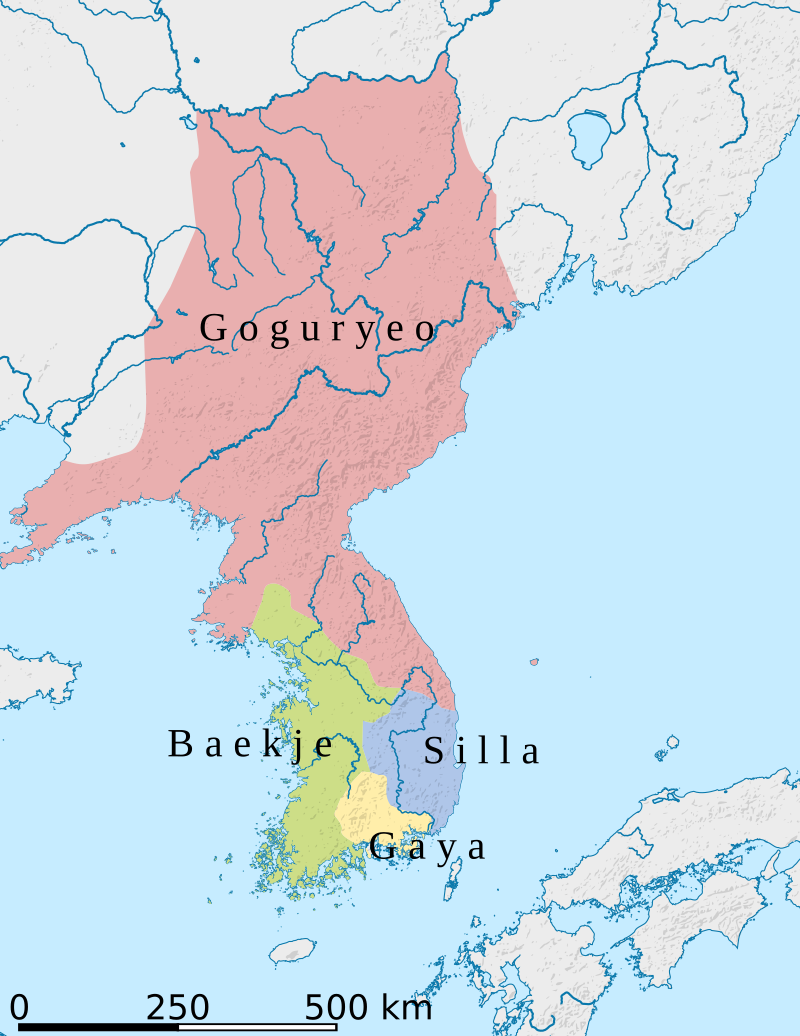
\includegraphics[width=0.3\textwidth]{images/Historia/mapa_tres_reinos.png} % Reemplaza 'mapa_corea' con el nombre de tu archivo de imagen
	\caption{Mapa de Corea con los Tres Reinos}
\end{figure}

\subsection{Goguryeo}

Goguryeo fue el reino más septentrional y poderoso de los Tres Reinos. Su capital estaba ubicada en la actual región norcoreana. Goguryeo mantuvo una fuerte influencia militar y política en la península, y se caracterizó por su habilidad para resistir las invasiones chinas de la dinastía Han y luego de la dinastía Tang. Este reino desarrolló una cultura propia y estableció una gran parte de lo que hoy es Corea del Norte.

\subsection{Baekje}

Baekje ocupó la región suroeste de la península coreana, con su capital en lo que hoy es la ciudad de Seúl. Este reino tenía estrechos vínculos culturales y comerciales con China y Japón, lo que le permitió adoptar y difundir la influencia budista en la península. Baekje fue conocido por su avanzada cultura y arte, y contribuyó significativamente al desarrollo de la cultura coreana.

\subsection{Silla}

Silla, ubicado en la región sureste de Corea con su capital en Gyeongju, fue el último de los Tres Reinos en unificarse bajo un gobierno centralizado. Silla es famoso por su sistema de gobierno estable y su énfasis en la educación y la cultura. Durante esta época, se estableció el sistema de exámenes gubernamentales basado en el conocimiento confuciano, que influyó en gran medida en la administración pública de Corea durante siglos.

A medida que avanzaba la época de los Tres Reinos, se produjo una serie de conflictos y alianzas cambiantes entre los reinos, con episodios de unificación temporal y fragmentación. Finalmente, en el siglo VII, Silla logró unificar la península coreana bajo su dominio y estableció el período conocido como el ''Silla Unificado``. Este período dio paso a una mayor estabilidad y desarrollo cultural en Corea antes de la llegada de la dinastía Goryeo. La época de los Tres Reinos dejó un profundo legado en la historia y la cultura de Corea, con influencias que perduran hasta el día de hoy.

\section{Hwarang}

Los \textbf{Hwarang}, también conocidos como ''Hwa Rang`` o ''Hwarangdo\textregistered``, fueron un grupo de jóvenes guerreros aristocráticos en la antigua Corea. Su existencia se sitúa en los períodos de los Tres Reinos y la posterior dinastía Silla, que abarcan los siglos VI al X d.C. Estos guerreros eran conocidos no sólo por su habilidad en el combate, sino también por su énfasis en la educación, la moral, la cultura y las artes.

\begin{figure}[h]
	\centering
	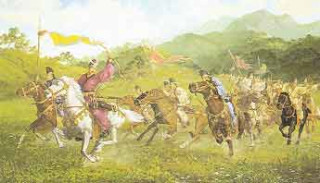
\includegraphics[width=0.3\textwidth]{images/Historia/pintura_hrd.jpg} % Reemplaza 'mapa_corea' con el nombre de tu archivo de imagen
	\caption{Grupo élite de Corea}
\end{figure}


\subsubsection{Origen y Significado}

La palabra ''Hwarang`` se traduce aproximadamente como ``caballeros de la flor'' o ``juventud floreciente''. Eran un grupo selecto de jóvenes nobles que se sometían a un entrenamiento riguroso tanto en artes marciales como en aspectos culturales y éticos.

\subsubsection{Educación Integral}

Los Hwarang no solo se entrenaban en técnicas de combate, sino que también recibían una educación completa que incluía poesía, música, filosofía y moral. Este enfoque en la educación y la cultura los diferenciaba de otros guerreros de la época.

\subsubsection{Código de Ética}

\begin{table}[t]
	\caption{Código Hwarang}
	\begin{center}
		\begin{tabular}{ | m{2cm} | m{5cm} | m{5cm} | }
			\hline Número & Hangul & Traducción \\ \hline
			Il & 사군이충: Sa Gun I Chung & Lealtad a nuestra Patria \\
			I & 사친이효: Sa Chin I Hyo & Lealtad a nuestros padres y maestros \\
			Sam & 교우이신: Gyo U I Sin & Confianza y hermandad entre amigos\\
			Sa & 임전무퇴: Im Jeon Mu Toe & Coraje para no retroceder frente al enemigo\\
			O & 살생유택: Sal Saeng Yu Taek & Justicia para no tomar una vida sin causa\\ \hline
		\end{tabular}
	\end{center}
\end{table}


Los Hwarang seguían un estricto código de ética conocido como ''Hwarangdo\textregistered``, que promovía valores como la lealtad, la rectitud, la valentía y la integridad. Este código tenía como objetivo formar no solo guerreros hábiles, sino también líderes virtuosos.

El fervor de los Hwarang ayudó a que Silla se convirtiera en la primera ''Tierra de Buda`` del mundo y condujo a la unificación de los tres reinos de Corea. Los principios budistas estaban tan arraigados en el código de los Hwarang que un gran número de monjes participaba en el Hwarang-Do, y durante tiempos de guerra, se despojaban de sus hábitos y tomaban las armas para morir por Silla.

El código Hwarang fue establecido en el trigésimo año del reinado del Rey Chin-Hung. Dos destacados guerreros Hwarang, Kwi-San y Ch'u-Hang, buscaron al famoso guerrero y monje budista Wong-Gwang Popsa en el Templo Kusil en la Montaña Unmun y le pidieron que les diera mandamientos que los hombres pudieran seguir y que no abrazaran la vida recluida de un monje budista.

\begin{figure}[h]
	\centering
	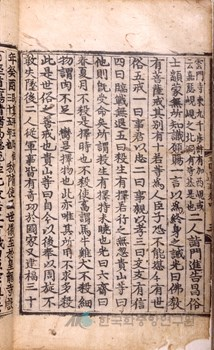
\includegraphics[width=0.4\textwidth]{images/Historia/codigo_hwarang.jpg} % Reemplaza 'mapa_corea' con el nombre de tu archivo de imagen
	\caption{Las Cinco Reglas Seculares de la Escuela de Wongwang en la época de los 3 reinos}
\end{figure}

Los mandamientos, basados en principios confucianos y budistas, se dividieron en el Código de las cinco reglas Hwarang y las nueve virtudes. Estos principios no eran tomados a la ligera por los Hwarang.


\begin{table}[t]
	\caption{Nueve Virtudes}
	\begin{center}
		\begin{tabular}{ | m{2cm} | m{5cm} | }
			\hline Hangul & Traducción \\ \hline
			인: In & Humanidad \\
			의: Ui & Justicia \\
			예: Ye & Cortesía \\
			지: Ji & Sabiduría \\
			신: Sin & Confianza \\
			선: Seon & Bondad \\
			덕: Deok & Virtud \\
			충: Chung & Lealtad \\
			용: Yong & Coraje \\

			\hline
		\end{tabular}
	\end{center}
\end{table}


El fervor de los Hwarang ayudó a que Silla se convirtiera en la primera "Tierra de Buda" del mundo y condujo a la unificación de los tres reinos de Corea. Los principios budistas estaban tan arraigados en el código de los Hwarang que un gran número de monjes participaban en el Hwarang-Do, y durante tiempos de guerra, se despojarían de sus hábitos y tomarían las armas para morir por Silla.

\subsubsection{Artes Marciales}

Aunque se destacaban en la educación y la cultura, los Hwarang también eran conocidos por su habilidad en el combate. Dominaban varias formas de artes marciales y estaban preparados para defender su reino en caso de guerra.

\subsubsection{Contribución a la Unificación de Silla}

Durante el período de los Tres Reinos en Corea, Silla se convirtió en uno de los reinos más poderosos. Se dice que los Hwarang desempeñaron un papel crucial en la unificación de Silla y en la posterior estabilidad del reino.

\subsubsection{Legado Cultural}

La influencia de los Hwarang perduró en la cultura coreana a lo largo de la historia. Su énfasis en la educación, la ética y la excelencia en las artes marciales influyó en la formación de la cultura y la identidad coreanas.

Los Hwarang son un ejemplo único en la historia de las sociedades guerreras, ya que combinaron la destreza en el combate con un profundo compromiso con la educación y los valores morales. Su legado sigue siendo un símbolo importante de la historia y la cultura coreanas.


%\begin{figure}[h]
%	\centering
%
%	\subfloat[Imagen 1]{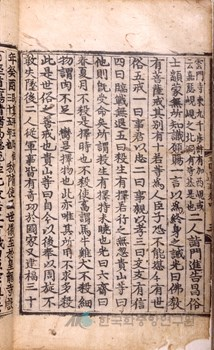
\includegraphics[width=0.2\textwidth]{images/Historia/codigo_hwarang.jpg}}\hspace{1cm}
%	\subfloat[Imagen 2]{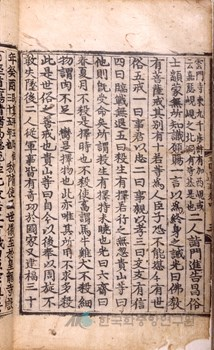
\includegraphics[width=0.2\textwidth]{images/Historia/codigo_hwarang.jpg}}\hspace{1cm}
%	\subfloat[Imagen 3]{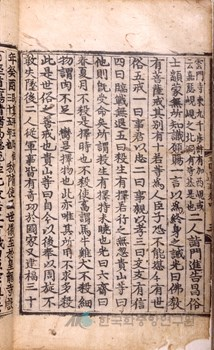
\includegraphics[width=0.2\textwidth]{images/Historia/codigo_hwarang.jpg}}\hspace{1cm}
%	\subfloat[Imagen 4]{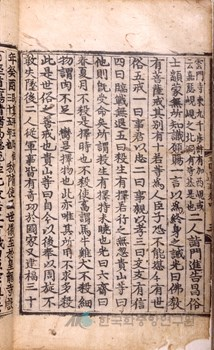
\includegraphics[width=0.2\textwidth]{images/Historia/codigo_hwarang.jpg}}\hspace{1cm}
%	\subfloat[Imagen 5]{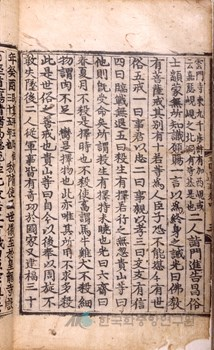
\includegraphics[width=0.2\textwidth]{images/Historia/codigo_hwarang.jpg}}
%
%	\caption{Secuencia Patada Frontal}
%
%\end{figure}

	\chapter{Vocabulario Coreano-Español}

En este capítulo, exploraremos algunas palabras y frases en coreano junto con sus traducciones al español. A continuación, encontrarás una lista de vocabulario básico.

\section{Saludos}

\begin{itemize}
	\item \textbf{안녕하세요 (Annyeong haseyo)} - Hola.
	\item \textbf{안녕 (Annyeong)} - Hola (informal).
	\item \textbf{안녕히 가세요 (Annyeonghi gaseyo)} - Adiós (cuando alguien se va).
	\item \textbf{안녕히 오세요 (Annyeonghi oseyo)} - Bienvenido (cuando alguien llega).
\end{itemize}

\section{Números}

Existen dos sistemas de numeración en Corea: el sistema nativo y el sistema sino-coreano. El sistema nativo se utiliza en contextos tradicionales y culturales, mientras que el sistema sino-coreano se usa en la mayoría de las situaciones modernas.

\begin{table}[t]
	\caption{Sistema de Numeración}
	\begin{center}
		\begin{tabular}{ | m{2cm} | m{5cm} | m{5cm} | }
			\hline Número & Sino-Coreano & Nativo\\ \hline
			0 & 영, 령 / 공 yeong, ryeong / gong &  \\
			1 & 일 il & 하나 hana \\
			2 & 이 i & 둘 dul \\
			3 & 삼 sam & 셋 set \\
			4 & 사 sa & 넷 net\\
			5 & 오 o & 다섯 daseot\\
			6 & 육 yuk & 여섯 yeoseot\\
			7 & 칠 chil & 일곱 ilgop\\
			8 & 팔 pal & 여덟 yeodeol \\
			9 & 구 gu & 아홉 ahop \\
			10 & 십 sip-il & 열 yeol\\
			11 & 십일 sip-il & 열 yeol-hana \\
			20 & 이십 i-sip & 열 seumul\\
			100 & 백 baek & \\
			1000 & 천 cheon & \\
			10000 & 백 man & \\ \hline
		\end{tabular}
	\end{center}
\end{table}

El uso del sitema Sino-Coreano se utiliza para:

\begin{itemize}
	\item Dar un número de teléfono
	\item Número de habitación
	\item Cálculos
	\item Dinero
	\item Años
	\item Siglos
	\item Número de páginas
\end{itemize}

Mientras que el uso del sistema nativo se usa para

\begin{itemize}
	\item Contar objetos
	\item Contar personas
	\item Decir la edad
	\item Hasta 99
\end{itemize}

\citeA{como-contar-en-coreano}



% Fuente: https://www.monash.edu/arts/languages-literatures-cultures-linguistics/korean-studies-research-hub/research/murksrh-language-lab/topic-1-how-to-know-when-to-use-pure-korean-vs-sino-korean-numbers


\section{Ad-Hoc}

%	경례 %% Saludo
%	검 %% Espada
\begin{itemize}
	\item \textbf{경례 (Hana)} - Saludo.
	\item \textbf{검 (Geom)} - Espada.
	\item \textbf{주먹 (Jumeok)} - Puño.
	\item \textbf{발차기 (Balchagi)} - Patada.
	\item \textbf{바닥 쓸기 (Badak Sseulgi)} - Barrido.
	\item \textbf{주먹질 (Jumeokjil)} - Golpear con el puño.
	\item \textbf{발차기 하다 (Balchagi Hada)} - Hacer una patada.
	\item \textbf{바닥 쓸기 하다 (Badak Sseulgi Hada)} - Realizar un barrido.
	\item \textbf{팔꿈치 (Palkkumchi)} - Codo.
	\item \textbf{무릎 (Mureup)} - Rodilla.
	\item \textbf{머리 (Meori)} - Cabeza.
	\item \textbf{몸 (Mom)} - Cuerpo.
	\item \textbf{방패 (Bangpae)} - Escudo.
	\item \textbf{방어 (Bang-eo)} - Defensa.
	\item \textbf{공격 (Gonggyeok)} - Ataque.
	\item \textbf{전투 (Jeontu)} - Combate.
	\item \textbf{킥 (Kick)} - Patada.
	\item \textbf{킥박스 (Kickbokseu)} - Kickboxing.
	\item \textbf{격투기 (Gyeoktugi)} - Artes marciales.
	\item \textbf{격투수 (Gyeoktu su)} - Luchador.
	\item \textbf{싸움 (Ssaum)} - Pelea.
	\item \textbf{방어 기술 (Bang-eo gisul)} - Técnicas de defensa.
	\item \textbf{공격 기술 (Gonggyeok gisul)} - Técnicas de ataque.
	\item \textbf{도장 (Dojang)} - Lugar de entrenamiento.
	\item \textbf{훈련 (Hunlyeon)} - Entrenamiento.
	\item \textbf{도복 (Dobok)} - Uniforme de artes marciales.
	\item \textbf{격투 무술 (Gyeoktu musul)} - Artes marciales.
	\item \textbf{급 (Geup)} - Grado (como en cinturón).
	\item \textbf{검도 (Geomdo)} - Esgrima.
	\item \textbf{권술 (Gwonsool)} - Defensa personal.

\end{itemize}


\section{Partes del Cuerpo}

\begin{itemize}
	\item \textbf{머리 (Meori)} - Cabeza.
	\item \textbf{목 (Mok)} - Cuello.
	\item \textbf{어깨 (Eokkae)} - Hombro.
	\item \textbf{가슴 (Gaseum)} - Pecho.
	\item \textbf{팔 (Pal)} - Brazo.
	\item \textbf{손 (Son)} - Mano.
	\item \textbf{손목 (Sonmok)} - Muñeca.
	\item \textbf{손가락 (Songarak)} - Dedo.
	\item \textbf{등 (Deung)} - Espalda.
	\item \textbf{허리 (Heori)} - Cintura.
	\item \textbf{배 (Bae)} - Abdomen.
	\item \textbf{다리 (Dari)} - Pierna.
	\item \textbf{무릎 (Mureup)} - Rodilla.
	\item \textbf{발 (Bal)} - Pie.
	\item \textbf{발목 (Balmok)} - Tobillo.
	\item \textbf{발가락 (Balgarak)} - Dedo del pie.
	\item \textbf{머리카락 (Meorikarak)} - Cabello.
	\item \textbf{눈 (Nun)} - Ojo.
	\item \textbf{귀 (Gwi)} - Oído.
	\item \textbf{입 (Ip)} - Boca.
	\item \textbf{이 (I)} - Diente.
	\item \textbf{혀 (Hyeo)} - Lengua.
	\item \textbf{코 (Ko)} - Nariz.
	\item \textbf{입술 (Ipsul)} - Labio.
	\item \textbf{턱 (Teok)} - Barbilla.
\end{itemize}
	\chapter{Programa de Entrenamiento de Hwarangdo\textregistered}

En esta sección, exploraremos el fascinante mundo del Hwarangdo\textregistered, un arte marcial que se caracteriza por su enfoque en las técnicas de combate y la disciplina física y mental. El Hwarangdo\textregistered es conocido por su variedad de movimientos y estilos, y en esta sección, te guiaremos a través de las técnicas clave que componen esta disciplina.

Las técnicas de Hwarangdo\textregistered se dividen en diferentes categorías, cada una con su enfoque particular. A continuación, presentamos una selección de técnicas organizadas de acuerdo a estas categorías para facilitar tu aprendizaje y comprensión:

\begin{enumerate}
	\item Técnicas de golpeo
	\item Técnicas de bloqueo
	\item Técnicas de patadas
	\item Técnicas de agarre y control
	\item Técnicas de defensa personal
\end{enumerate}

A lo largo de esta sección, te proporcionaremos una descripción detallada de cada técnica, así como instrucciones paso a paso sobre cómo realizarlas correctamente. Además, encontrarás consejos y recomendaciones para mejorar tu técnica y tu comprensión de Hwarangdo\textregistered.

Ya seas un principiante que está dando sus primeros pasos en el Hwarangdo\textregistered o un practicante experimentado en busca de refinar sus habilidades, esta sección está diseñada para brindarte información valiosa y recursos que te ayudarán en tu viaje de entrenamiento.

Los practicantes de Hwarangdo\textregistered avanzan a través de niveles de expertise que se distinguen por colores. Cada nivel tiene requisitos específicos que los estudiantes deben cumplir para avanzar al siguiente. A medida que progresas en tu entrenamiento, es fundamental dominar las técnicas correspondientes a tu nivel actual para alcanzar nuevos desafíos y objetivos en tu camino hacia la maestría en Hwarangdo\textregistered.

A continuación, detallaremos los niveles de expertise y las técnicas clave que deben dominar los practicantes para avanzar:


\section{Nivel Blanco}


\subsection[Duración]{Tiempo Estimado}

Tiempo estimado de entrenamiento es de 24 a 36 horas

\subsection{Requerimientos para optar a faja celeste}


\begin{table}[t]
	\caption{Curso Faja Blanca}
	\begin{center}
		\begin{tabular}{ | m{2cm} | m{5cm} | m{5cm} | }
			\hline Detalle & Descripión & Listado\\ \hline
			Soo gi sul dae ryun & Técnicas de puños libres & N°1 al N°5\\
			Kwon bop & Defensa Tradicional & N°1 al N°5\\
			Palkoop sul & Técnicas básicas de codo & N°1 al N°7\\
			Soo Do il bang & Mano de espada/Posición de dragón & N°1 al N°3\\
			Mu Kom sul & Técnica básica espada de madera & N°1 al N° 5\\ \hline
		\end{tabular}
	\end{center}
\end{table}


Los estudiantes deberán superar un examen para avanzar al siguiente nivel.

\section{Nivel Celeste}

Este color representa el cielo, el empezar a soñar y comenzar la búsqueda para superarse

\subsection[Duración]{Tiempo Estimado}

Tiempo estimado de entrenamiento es de 24 a 36 horas

\subsection{Requerimientos para optar a faja Celeste-Amarillo}

\begin{itemize}
	\item Puñetazos básicos
	\item Bloqueo de ataques simples
	\item Patadas frontales
	\item Postura y equilibrio adecuados
\end{itemize}

Los estudiantes deberán superar un examen para avanzar al siguiente nivel.

\section{Nivel Celeste-Amarillo}
Este color representa el sol en el cielo, el empezar a comenzar a comprender las técnicas. El amanecer

\subsection[Duración]{Tiempo Estimado}

Tiempo estimado de entrenamiento es de 24 a 36 horas

\subsection{Requerimientos para optar a faja Amarillo}

\begin{itemize}
	\item Puñetazos básicos
	\item Bloqueo de ataques simples
	\item Patadas frontales
	\item Postura y equilibrio adecuados
\end{itemize}

Los estudiantes deberán superar un examen para avanzar al siguiente nivel.

\section{Nivel Amarillo}

Este color representa el sol y la habilidades adquiridas.

\subsection[Duración]{Tiempo Estimado}

Tiempo estimado de entrenamiento es de 24 a 36 horas

\subsection{Requerimientos para optar a faja Amarillo-Verde}

\begin{itemize}
	\item Puñetazos básicos
	\item Bloqueo de ataques simples
	\item Patadas frontales
	\item Postura y equilibrio adecuados
\end{itemize}

Los estudiantes deberán superar un examen para avanzar al siguiente nivel.

\section{Nivel Amarillo-Verde}

Representa el crecimiento de un árbol y a la vez en el alumno sus raíces en el sistema

\subsection[Duración]{Tiempo Estimado}

Tiempo estimado de entrenamiento es de 24 a 36 horas

\subsection{Requerimientos para optar a faja Verde}

\begin{itemize}
	\item Puñetazos básicos
	\item Bloqueo de ataques simples
	\item Patadas frontales
	\item Postura y equilibrio adecuados
\end{itemize}

Los estudiantes deberán superar un examen para avanzar al siguiente nivel.


\section{Nivel Verde}

Representa un árbol alimentándose de agua, nutriendo sus raíces. El alumno se aplica en el conocimiento y desarrollo interno

\subsection[Duración]{Tiempo Estimado}

Tiempo estimado de entrenamiento es de 24 a 36 horas

\subsection{Requerimientos para optar a faja Verde-Azul}

\begin{itemize}
	\item Puñetazos básicos
	\item Bloqueo de ataques simples
	\item Patadas frontales
	\item Postura y equilibrio adecuados
\end{itemize}

Los estudiantes deberán superar un examen para avanzar al siguiente nivel.

\section{Nivel Verde-Azul}

Representa un árbol alimentándose de agua, nutriendo sus raíces. El alumno se aplica en el conocimiento y desarrollo interno

\subsection[Duración]{Tiempo Estimado}

Tiempo estimado de entrenamiento es de 24 a 36 horas

\subsection{Requerimientos para optar a faja Azul}

\begin{itemize}
	\item Puñetazos básicos
	\item Bloqueo de ataques simples
	\item Patadas frontales
	\item Postura y equilibrio adecuados
\end{itemize}

Los estudiantes deberán superar un examen para avanzar al siguiente nivel.

\section{Nivel Azul}

Representa el agua con toda su fuerza. En el alumno aprende a amoldarse a todo tipo de situaciones de conflicto con suavidad o con mucha fuerza

\subsection[Duración]{Tiempo Estimado}

Tiempo estimado de entrenamiento es de 60 horas

\subsection{Requerimientos para optar a faja Roja}

\begin{itemize}
	\item Puñetazos básicos
	\item Bloqueo de ataques simples
	\item Patadas frontales
	\item Postura y equilibrio adecuados
\end{itemize}

Los estudiantes deberán superar un examen para avanzar al siguiente nivel.




¡Comencemos explorando estas emocionantes técnicas de Hwarangdo\textregistered y sumergiéndonos en el mundo de este apasionante arte marcial!

	\chapter{Técnicas de Puño}

El capítulo dedicado a las ``Técnicas de Puños'' es un componente fundamental en el entrenamiento de Hwarangdo\textregistered. En esta sección, los practicantes exploran el arte y la precisión de los golpes, desarrollando habilidades esenciales para la defensa personal y el combate. Desde los conceptos básicos de la postura y el equilibrio hasta la aplicación efectiva de golpes, este capítulo proporciona una base sólida para la comprensión de cómo canalizar la fuerza y la energía a través de los puños. Los estudiantes aprenderán la importancia de la técnica y la velocidad, así como la coordinación y la sincronización necesarias para ejecutar golpes poderosos y precisos. A medida que avancen en este capítulo, ganarán una apreciación más profunda de la importancia de la disciplina y la perseverancia en el camino hacia la maestría en Hwarangdo\textregistered.

\section{Empuñadura de la Mano}

\subsection{Empuñadura Cerrada}

La empuñadura cerrada es un estilo común en muchas disciplinas marciales. En esta técnica, los dedos se cierran firmemente alrededor del puño, con el pulgar cubriendo los nudillos. Esto proporciona un sólido punto de impacto y permite realizar golpes potentes y precisos.

\begin{figure}[h]
	\centering
	
\includegraphics[width=0.2\linewidth]{images/Técnicas/puno_cerrado.jpg}
	\caption{Empuñadura Cerrada}
\end{figure}

\subsection{Empuñadura Abierta}

La empuñadura abierta es más relajada en comparación con la empuñadura cerrada. Los dedos están extendidos y relajados, con el pulgar ligeramente doblado hacia adentro. Esta técnica se utiliza en situaciones donde se necesita más control y precisión, como en las técnicas de bloqueo y control.

\begin{figure}[h]
	\centering
	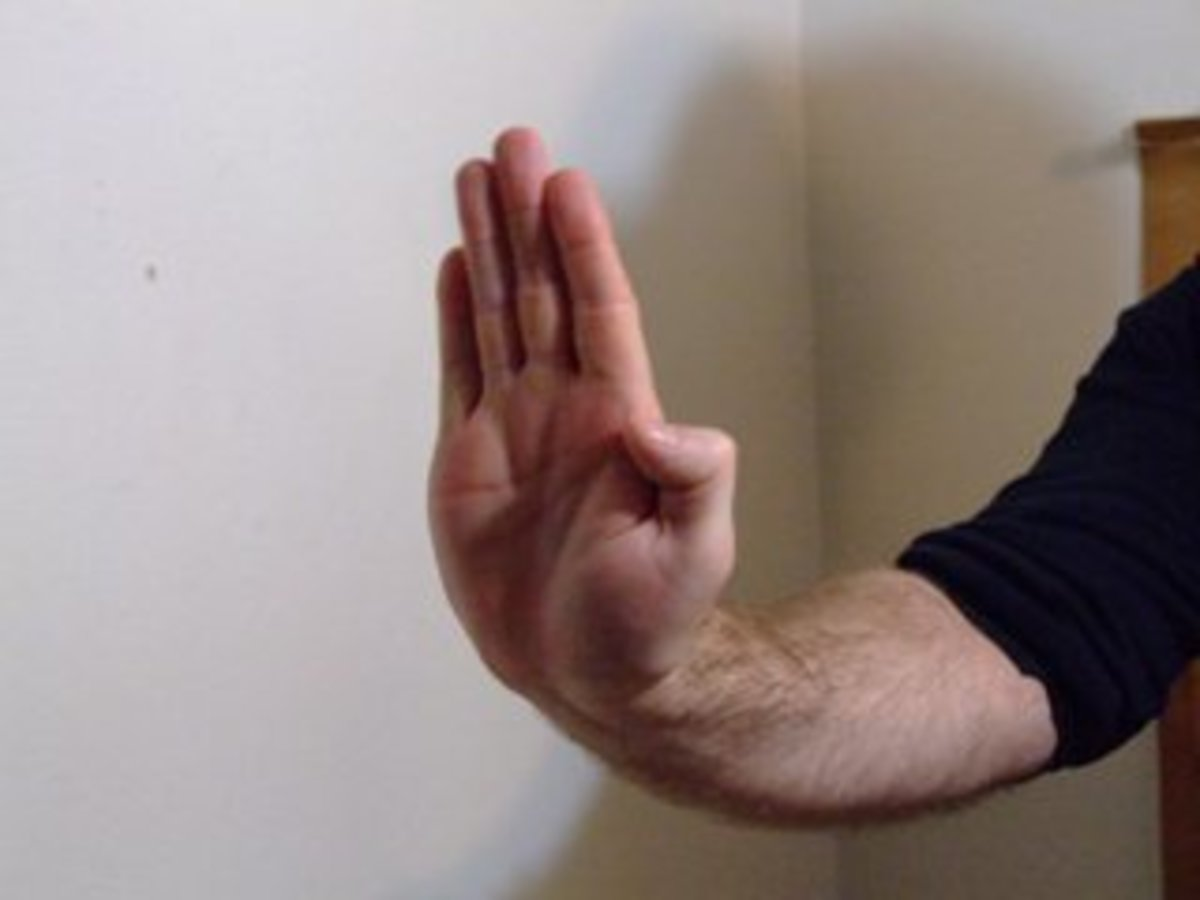
\includegraphics[width=0.2\linewidth]{images/Técnicas/puno_abierto.jpg}
	\caption{Empuñadura Abierta}
\end{figure}


	\chapter{Técnicas de Patadas}

El capítulo dedicado a las ``Técnicas de Patadas'' es una parte esencial del entrenamiento en Hwarangdo\textregistered. Aquí, los practicantes exploran la elegancia y la versatilidad de las patadas, desarrollando habilidades cruciales tanto en la defensa personal como en el combate. Desde las patadas básicas hasta las avanzadas, este capítulo ofrece una base sólida para comprender cómo utilizar las piernas de manera efectiva como herramientas de ataque y defensa. Los estudiantes aprenderán la importancia de la técnica, el equilibrio y la flexibilidad, así como la necesidad de adaptar las patadas a diferentes situaciones. A medida que avanzan en este capítulo, adquieren una apreciación más profunda de la precisión y la agilidad, elementos esenciales para dominar el arte de las patadas en Hwarangdo\textregistered. Este capítulo no solo les brinda una amplia gama de herramientas de combate, sino que también fomenta la disciplina y la perseverancia, impulsándolos hacia la maestría en esta apasionante disciplina marcial.


	\chapter{Técnicas del Monje Wong-Gwang Popsa}

El capítulo dedicado a las ``Técnicas del Monje Wong-Gwang Popsa'' representa un componente excepcionalmente valioso en el vasto repertorio de Hwarangdo\textregistered. Este enfoque singular se centra en la capacidad de responder de manera efectiva a un ataque del oponente a través de una combinación de bloqueo, esquiva y desvío de los golpes entrantes. Los practicantes de esta disciplina marcial aprenden a anticipar y contrarrestar las embestidas del oponente con precisión y agilidad.

Una vez que se ha neutralizado el ataque, el defensor responde con una serie de movimientos que pueden incluir proyecciones y retenciones en puntos específicos de articulación o puntos de presión, lo que añade una dimensión única al combate en Hwarangdo\textregistered. La maestría de estas técnicas no solo requiere habilidad física, sino también un profundo conocimiento de la anatomía humana y la capacidad de aprovechar la fuerza y el impulso del oponente en beneficio propio.

Este capítulo no solo imparte habilidades de autodefensa prácticas, sino que también promueve la agudeza mental y la adaptabilidad, ya que los practicantes deben tomar decisiones rápidas en situaciones de combate. La atención al detalle y la concentración son esenciales para el éxito en las Técnicas del Monje Wong-Gwang Popsa, lo que hace que esta área de Hwarangdo\textregistered sea una de las más desafiantes y gratificantes para aquellos que buscan dominar este antiguo arte marcial.

\section{Preámbulo}

\subsection{Técnica 1}

En la Figura \ref{fig:figura1} podemos ver un paisaje antes de la guerra. En la Figura \ref{fig:figura2} se muestra el mismo paisaje después de la guerra. El tratado X se llevó a cabo para resolver el conflicto, como se ilustra en la Figura \ref{fig:figura3}.
\lipsum[1]

%Mostrar una secuencia a 3 fotos por renglón
\begin{figure}[h]
	\centering
	\begin{minipage}{0.3\textwidth}
		
\includegraphics[width=\linewidth]{images/Técnicas/puno_cerrado.jpg}
		\caption{Paisaje antes de la guerra}
		\label{fig:figura1}
	\end{minipage}
	\hfill
	\begin{minipage}{0.3\textwidth}
		
\includegraphics[width=\linewidth]{images/Técnicas/puno_cerrado.jpg}
		\caption{Paisaje después de la guerra}
		\label{fig:figura2}
	\end{minipage}
	\hfill
	\begin{minipage}{0.3\textwidth}
		
\includegraphics[width=\linewidth]{images/Técnicas/puno_cerrado.jpg}
		\caption{Tratado X}
		\label{fig:figura3}
	\end{minipage}
\end{figure}



% Mostrar una secuencia a 2 fotos
%\begin{figure}[h]
%	\centering
%	\begin{minipage}{0.45\textwidth}
%		
\includegraphics[width=\linewidth]{images/Técnicas/puno_cerrado.jpg}
%		\caption{Paisaje antes de la guerra}
%		\label{fig:figura1}
%	\end{minipage}
%	\hfill
%	\begin{minipage}{0.45\textwidth}
%		
\includegraphics[width=\linewidth]{images/Técnicas/puno_cerrado.jpg}
%		\caption{Paisaje después de la guerra}
%		\label{fig:figura2}
%	\end{minipage}
%	\hfill
%	%	\begin{minipage}{0.3\textwidth}
%	%		
\includegraphics[width=\linewidth]{images/Técnicas/puno_cerrado.jpg}
%	%		\caption{Tratado X}
%	%		\label{fig:figura3}
%	%	\end{minipage}
%\end{figure}







	\chapter{Lucha de Piso}

La lucha de piso es un aspecto emocionante y esencial en la formación de jóvenes artistas marciales. A menudo subestimada, esta disciplina desempeña un papel crucial en el desarrollo de habilidades fundamentales tanto en la defensa personal como en los deportes de combate. En este capítulo, nos sumergiremos en el apasionante mundo de la lucha de piso, adaptándola a un nivel escolar y destinada a jóvenes menores de 18 años.

Desde las técnicas básicas de caída y control hasta las maniobras de sumisión más simples, aquí aprenderemos los fundamentos que sientan las bases para un crecimiento sólido en las artes marciales. Además de las habilidades técnicas, exploraremos la importancia de la disciplina, el respeto y la autoconfianza que la lucha de piso puede inculcar en nuestros jóvenes practicantes.

Descubriremos cómo la lucha de piso se adapta de manera segura y efectiva al entorno escolar, promoviendo valores como la cooperación, el trabajo en equipo y el autocontrol. Aprenderemos cómo estas habilidades pueden ser aplicadas en situaciones de la vida cotidiana y cómo el entrenamiento constante fomenta el respeto por sí mismo y por los demás.

Este capítulo está diseñado para empoderar a nuestros jóvenes practicantes y ayudarlos a desarrollar habilidades físicas y mentales esenciales. Preparaos para embarcaros en un emocionante viaje de autodescubrimiento y crecimiento a través de la lucha de piso, brindando a nuestros jóvenes las herramientas necesarias para enfrentar los desafíos de la vida con confianza y determinación.

¡Comencemos nuestro viaje en el apasionante mundo de la lucha de piso adaptada a jóvenes menores de 18 años!

\section{Preámbulo}

En esta sección, exploraremos los fundamentos esenciales de la lucha de piso y lo que necesitas para comenzar. La lucha de piso es una disciplina emocionante que requiere una preparación adecuada y un conjunto específico de elementos para practicar de manera segura y efectiva.

\begin{itemize}
	\item \textbf{Piso Apropiado:} Un piso adecuado es fundamental para la práctica segura de la lucha de piso. Se recomienda utilizar tatamis o superficies acolchadas que ayuden a absorber el impacto de las caídas y minimicen el riesgo de lesiones. Asegúrate de que el área de entrenamiento esté libre de objetos afilados o peligrosos.

	\item \textbf{Ropa Apropiada:} La elección de la ropa es importante para garantizar la comodidad y la seguridad durante la lucha de piso. Se recomienda el uso de un uniforme de artes marciales adecuado, que suele consistir en un gi (chaqueta y pantalones) y un cinturón para atar la chaqueta. Además, se deben llevar ropa interior adecuada y asegurarse de que el uniforme esté limpio y en buenas condiciones.

	\item \textbf{Jueces y Supervisión:} En la lucha de piso, es esencial contar con jueces o supervisores que puedan observar y evaluar las técnicas y el comportamiento de los participantes. Los jueces deben estar capacitados para hacer cumplir las reglas y garantizar que se mantenga un ambiente seguro y respetuoso durante la práctica o la competición.

	\item \textbf{Normas y Reglas:} Es importante establecer normas y reglas claras para la lucha de piso, que definan qué técnicas son permitidas y cuáles no, así como las pautas de conducta esperadas de los participantes. Las reglas pueden variar según el estilo o la organización, por lo que es fundamental conocerlas y seguirlas en todo momento.

	\item \textbf{Socios de Entrenamiento:} En la lucha de piso, es común practicar con socios de entrenamiento. Selecciona a tus socios con cuidado y asegúrate de que estén igualmente comprometidos con la seguridad y el respeto mutuo. La comunicación con tus socios es fundamental para garantizar una práctica efectiva y segura.

	\item \textbf{Equipo de Protección (Opcional):} Aunque no es siempre obligatorio, el uso de equipo de protección como protectores bucales y protectores de oídos puede ayudar a prevenir lesiones menores durante la lucha de piso. Considera su uso, especialmente en entrenamientos más intensos.
\end{itemize}

\section{Objetivos}

La lucha de piso es una disciplina marcial que va más allá de la fuerza bruta y la agresión. Requiere habilidades técnicas, resistencia física y mental, así como una comprensión profunda de la estrategia. En este capítulo, exploraremos los objetivos fundamentales de la lucha de piso, con un énfasis especial en el desarrollo del control, y cómo esta disciplina puede enriquecer tu viaje en las artes marciales.

\begin{itemize}
	\item \textbf{Desarrollo de Técnicas de Control:} El objetivo principal de la lucha de piso es aprender a controlar y someter a un oponente en el suelo. Esto incluye el dominio de técnicas de inmovilización y sumisión, donde el control es esencial.

	\item \textbf{Mejora de la Resistencia Física:} La lucha de piso requiere una gran resistencia física para mantener el control durante los combates prolongados. El entrenamiento constante contribuye al desarrollo de la resistencia cardiovascular, la fuerza muscular y la agilidad.

	\item \textbf{Fomento de la Autodisciplina:} El control sobre uno mismo y la autodisciplina son fundamentales en la lucha de piso. Los practicantes aprenden a mantener la calma y tomar decisiones estratégicas incluso en situaciones de alta presión.

	\item \textbf{Desarrollo de la Conciencia Corporal:} Entender la posición y movimiento del propio cuerpo es esencial en la lucha de piso, especialmente para mantener el control sobre el oponente. Esto se traduce en una mayor conciencia corporal y coordinación.

	\item \textbf{Mejora de la Toma de Decisiones:} La lucha de piso implica tomar decisiones rápidas y efectivas en tiempo real, especialmente en situaciones de control. Esta habilidad se aplica no solo en el tatami, sino también en la vida cotidiana.

	\item \textbf{Promoción del Respeto y la Humildad:} El control sobre la propia fuerza y el respeto por los oponentes y compañeros de entrenamiento son una parte integral de la lucha de piso. Fomenta la humildad y la cortesía en el trato con los demás.

	\item \textbf{Aplicación en la Defensa Personal:} Las habilidades de control en la lucha de piso son útiles en situaciones de defensa personal, donde la capacidad de controlar a un oponente puede ser crucial.

	\item \textbf{Participación en Competiciones:} Para aquellos interesados en competir, la lucha de piso ofrece la oportunidad de probar sus habilidades en torneos y competiciones, donde el control es una habilidad vital.

	\item \textbf{Disfrute y Crecimiento Personal:} Por encima de todo, la lucha de piso es una fuente de disfrute y crecimiento personal, donde el control sobre uno mismo y los demás enriquece la vida en muchas formas.
\end{itemize}


\section{Reglas de la Lucha de Piso Escolar}

Las reglas de la lucha de piso escolar están diseñadas para promover la seguridad de los participantes y enfatizar la inmovilización como objetivo principal. A continuación se detallan las reglas básicas:

\begin{enumerate}
	\item \textbf{Objetivo de la Lucha:} El ganador es quien logra inmovilizar al oponente de espalda en el suelo en una posición dominadora durante un período de tiempo específico, generalmente 10 segundos o más.

	\item \textbf{Puntuación:} La victoria se determina cuando uno de los luchadores inmoviliza con éxito al oponente durante el tiempo requerido (10 segundos o más) mientras mantiene una posición dominante.

	\item \textbf{Prohibición de Técnicas de Estrangulación y Torción:} Está estrictamente prohibido aplicar cualquier tipo de estrangulación, torción o asfixia sobre el oponente. El enfoque principal debe ser la inmovilización y el control, no causar daño físico al oponente.

	\item \textbf{Énfasis en la Seguridad:} La seguridad de los participantes es primordial. Los estudiantes deben practicar bajo la supervisión de un instructor experimentado y deben estar familiarizados con las técnicas de caída segura y la prevención de lesiones.

	\item \textbf{Respeto y Cortesía:} Se espera que los participantes muestren respeto y cortesía hacia sus oponentes. Esto incluye respetar las señales de rendición del oponente y seguir las instrucciones del árbitro o instructor.

\end{enumerate}


\section{Iniciando la Lucha de Piso}

La lucha de piso comienza con un ritual de respeto y preparación que establece el tono para el entrenamiento o el combate. A continuación, se describen los pasos clave para iniciar la lucha de piso, ilustrados con fotografías de referencia.

\subsection*{Paso 1: Saludo Budista}

En la primera etapa, los practicantes se colocan a una distancia de aproximadamente un metro el uno del otro, manteniendo una postura de respeto y concentración. El saludo budista tradicional es un gesto de cortesía que demuestra respeto mutuo y armonía. Las manos se unen en una posición de colocar la palma izquierda sobre el piso, luego la mano derecha, con los dedos, cubre el área con los otro, y llevando la frente sobre las manos. Esta es una muestra de gratitud y respeto hacia el oponente y hacia las enseñanzas de las artes marciales. Se ilustra en la Figura \ref{saludo_budista_lp}.

\begin{figure}[h]
	\centering
	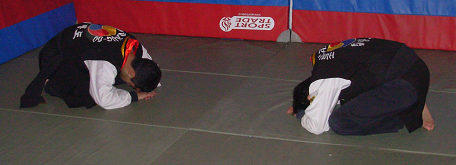
\includegraphics[width=0.5\textwidth]{images/Lucha_de_Piso/01_saludo.png}
	\caption{Saludo Budista Tradicional}
	\label{fig:saludo_budista_lp}
\end{figure}

\subsection*{Paso 2: Saludo Occidental Modificado}

Después del saludo budista, los practicantes pueden realizar un saludo occidental modificado, que es un gesto de cortesía occidental con un toque marcial. En este saludo, la mano izquierda se coloca debajo del brazo derecho extendido hacia adelante. Esta posición muestra respeto y preparación para el combate. Se ilustra en la Figura \ref{fig:saludo_occidental_lp}.

\begin{figure}[h]
	\centering
	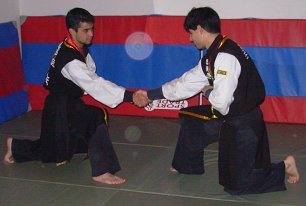
\includegraphics[width=0.5\textwidth]{images/Lucha_de_Piso/02_saludo_mano.png}
	\caption{Saludo Occidental Modificado}
	\label{fig:saludo_occidental_lp}
\end{figure}

\subsection*{Paso 3: Posición Inicial}

Una vez completados los saludos, los practicantes adoptan una posición inicial que varía según el estilo de lucha de piso. La posición inicial es fundamental para mantener el equilibrio y la preparación para cualquier movimiento. Se ilustra en la Figura \ref{fig:posicion_inicial_lp}.

\begin{figure}[h]
	\centering
	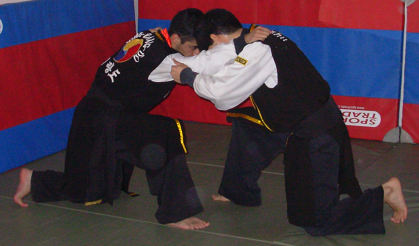
\includegraphics[width=0.5\textwidth]{images/Lucha_de_Piso/03_posicion_inicial.png}
	\caption{Posición Inicial}
	\label{fig:posicion_inicial_lp}
\end{figure}

Estos pasos iniciales establecen un ambiente de respeto y concentración, y preparan a los practicantes para la acción en la lucha de piso. Desde esta posición inicial, comienza la exploración de técnicas y estrategias esenciales en este emocionante aspecto de las artes marciales.


Es fundamental que los participantes comprendan y respeten estas reglas para garantizar un ambiente seguro y respetuoso durante la práctica de la lucha de piso escolar.

\subsection{Técnicas básicas de inmovilización}

¡Comencemos a explorar las técnicas básicas de inmovilización en la lucha de piso y a desarrollar tus habilidades en esta emocionante disciplina de las artes marciales!


\begin{enumerate}
	\item \textbf{Inmovilización Lateral:}

	\begin{itemize}
		\item Posición Inicial: En la Montada en Posición Crucifijo, un competidor se encuentra encima de su oponente, utilizando su propio cuerpo para presionar el pecho del oponente.

		\item Orientación Corporal: Quien está arriba adopta la posición boca arriba, mientras que el oponente está posicionado boca abajo en el suelo. Esta disposición inicial crea una ventaja estratégica para el luchador en la parte superior.

		\item Posición Perpendicular: La característica distintiva de esta técnica es que el practicante que está arriba se coloca de manera perpendicular al cuerpo del oponente. Esto significa que su torso atraviesa el torso del oponente en un ángulo de 90 grados, lo que le proporciona un control efectivo. Ver \ref{fig:posicion_lateral_frontal_lp}

		\item Rodilla bajo el Brazo: Además, quien está arriba posiciona una de sus rodillas debajo del brazo del oponente que está abajo. Esta táctica bloquea el movimiento del brazo del oponente y restringe sus opciones de defensa. Ver \ref{fig:posicion_lateral_lateral_lp}
	\end{itemize}

	% Mostrar una secuencia a 2 fotos
	\begin{figure}[h]
		\centering
		\begin{minipage}{0.45\textwidth}
			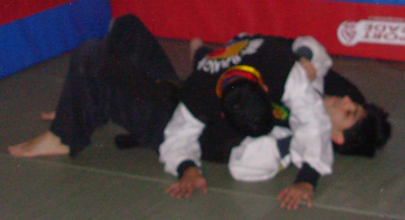
\includegraphics[width=\linewidth]{images/Lucha_de_Piso/04_posicion_lateral_a.png}
			\caption{Inmovilización lateral vista frontal}
			\label{fig:posicion_lateral_frontal_lp}
		\end{minipage}
		\hfill
		\begin{minipage}{0.45\textwidth}
			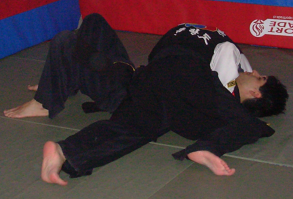
\includegraphics[width=\linewidth]{images/Lucha_de_Piso/05_posicion_lateral_b.png}
			\caption{Inmovilización lateral vista lateral}
			\label{fig:posicion_lateral_lateral_lp}
		\end{minipage}
		\hfill
	\end{figure}

	\item \textbf{Inmovilización de Pulpo:} El "Control del Pulpo" es una técnica de inmovilización en HwaRangDo que guarda similitudes con la anteriormente mencionada. La diferencia principal radica en que el oponente se encuentra sentado, ubicado cerca del hombro del practicante que ejecuta la técnica. A continuación, se detalla esta técnica: Ver \ref{fig:posicion_lateral_pulpo_lp}.

	\begin{itemize}
		\item Posición Inicial: El oponente se encuentra sentado, con su ubicación cercana al hombro del practicante que realiza la técnica.
		\item Abrazo de Brazos: Quien ejecuta la técnica rodea ambos brazos del oponente por detrás de su cabeza. Existen variantes en las que el practicante puede optar por cerrar la posición sujetando su propia corva o el cinturón del uniforme del oponente.
		\item Presión en el Pecho: El cuerpo del practicante que está arriba aplica presión sobre el pecho del oponente, restringiendo su capacidad de movimiento.
		\item Posición de las Piernas: Para mantener un control sólido, las piernas del practicante deben estar separadas y paralelas al suelo, asumiendo una forma abstracta que recuerda la de un pulpo.
	\end{itemize}

	\begin{figure}[h]
		\centering
		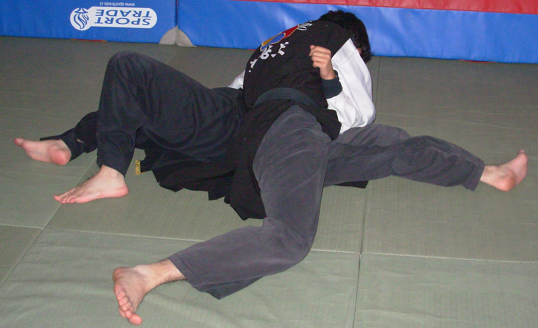
\includegraphics[width=0.5\textwidth]{images/Lucha_de_Piso/06_posicion_lateral_pulpo.png}
		\caption{Inmovilización de pulpo}
		\label{fig:posicion_lateral_pulpo_lp}
	\end{figure}


	\item \textbf{Inmovilización a una pierna:} En esta técnica de inmovilización, el ejecutor se coloca de manera perpendicular con respecto al oponente, quien puede estar boca arriba (Figura \ref{fig:inmovilizacion_una_pierna_frontal_lp}) o boca abajo en el suelo (Ver Figura \ref{fig:inmovilizacion_una_pierna_lateral_lp}). Los pasos clave son los siguientes:

	\begin{itemize}
		\item El ejecutor coloca uno de sus brazos por detrás de la nuca del oponente.
		\item El otro brazo se desliza por debajo de ambos muslos del oponente.
		\item Ambas manos del ejecutor intentan unirse para completar la inmovilización.
	\end{itemize}

	% Mostrar una secuencia a 2 fotos
	\begin{figure}[h]
		\centering
		\begin{minipage}{0.45\textwidth}
			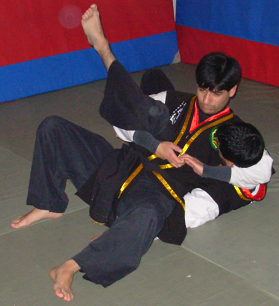
\includegraphics[width=\linewidth]{images/Lucha_de_Piso/07_inmovilizacion_a_una_pierna_frontal.png}
			\caption{Posición de inmovilización a una pierna boca arriba}
			\label{fig:inmovilizacion_una_pierna_frontal_lp}
		\end{minipage}
		\hfill
		\begin{minipage}{0.45\textwidth}
			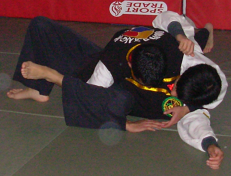
\includegraphics[width=\linewidth]{images/Lucha_de_Piso/08_inmovilizacion_a_una_pierna_lateral.png}
			\caption{Posición de inmovilización a una pierna boca abajo}
			\label{fig:inmovilizacion_una_pierna_lateral_lp}
		\end{minipage}
		\hfill
	\end{figure}

	\item \textbf{Inmovilización a dos piernas:} En esta técnica de inmovilización, el ejecutor se coloca de manera perpendicular con respecto al oponente, quien puede estar boca arriba (Figura \ref{fig:inmovilizacion_dos_piernas_frontal_lp}) o boca abajo en el suelo (Ver Figura \ref{fig:inmovilizacion_dos_piernas_lateral_lp}). Los pasos clave son los siguientes:

	\begin{itemize}
		\item El ejecutor coloca uno de sus brazos por detrás de la nuca del oponente.
		\item El otro brazo se desliza por debajo del muslo del oponente.
		\item Ambas manos del ejecutor intentan unirse para completar la inmovilización.
	\end{itemize}


	% Mostrar una secuencia a 2 fotos
	\begin{figure}[h]
		\centering
		\begin{minipage}{0.45\textwidth}
			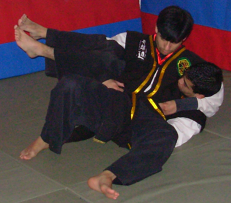
\includegraphics[width=\linewidth]{images/Lucha_de_Piso/09_inmovilizacion_a_una_pierna_lateral.png}
			\caption{Posición de retención lateral vista frontal}
			\label{fig:inmovilizacion_dos_piernas_frontal_lp}
		\end{minipage}
		\hfill
		\begin{minipage}{0.45\textwidth}
			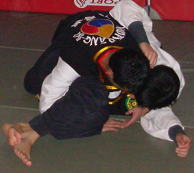
\includegraphics[width=\linewidth]{images/Lucha_de_Piso/10_inmovilizacion_a_una_pierna_lateral.png}
			\caption{Inmovilización lateral vista lateral}
			\label{fig:inmovilizacion_dos_piernas_lateral_lp}
		\end{minipage}
		\hfill
	\end{figure}



	\item \textbf{Inmovilización abrazo de cintura:} En esta técnica de inmovilización, el ejecutor abraza al oponente por la espalda a la altura de la cintura. Los pasos clave son los siguientes: Ver \ref{fig:posicion_abrazo_cintura}.

	\begin{itemize}
		\item El ejecutor rodea al oponente por la cintura con sus brazos, asegurando un agarre sólido.
		\item Luego, intenta bajar o acercar su propia cadera al suelo lo más posible.
		\item El pie que está más cerca del oponente se abre, y la parte interna de este pie queda tocando el suelo.
	\end{itemize}

	Esta técnica genera una especie de ''peso muerto`` que dificulta al oponente escapar, ya que el ejecutor tiene un control efectivo sobre su cintura y ha establecido una base sólida en el suelo.

	\begin{figure}[h]
		\centering
		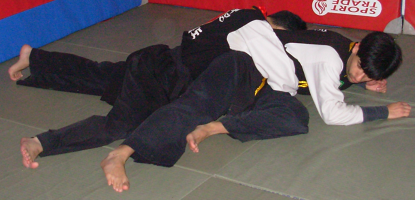
\includegraphics[width=0.5\textwidth]{images/Lucha_de_Piso/11_inmovilizacion_abrazo_cintura.png}
		\caption{Inmovilización de cintura}
		\label{fig:posicion_abrazo_cintura}
	\end{figure}

	\item \textbf{Inmovilización de montada} La inmovilización de montada en HwaRangDo se asemeja a la posición de un jinete montando a caballo. Los pasos clave de esta técnica son los siguientes: . Ver \ref{fig:posicion_montada}.

	\begin{itemize}
		\item \textbf{Posición del Ejecutor:} El practicante se coloca sobre el oponente, sentándose sobre su torso. Esta posición proporciona un control total sobre el oponente.
		\item \textbf{Unión del Pecho:} El ejecutor acerca su pecho al rostro del oponente, minimizando la capacidad de movimiento de este último.
		\item \textbf{Brazos detrás de la Cabeza:} Los brazos del practicante se juntan detrás de la cabeza del oponente. Esta posición no solo limita la capacidad de defensa del oponente, sino que también prepara el terreno para posibles estrangulamientos y sumisiones.
	\end{itemize}

	La inmovilización de montada es una posición de control fundamental en el Jiu-Jitsu, que permite al practicante dominar y mantener al oponente en el suelo mientras busca oportunidades para someterlo o avanzar hacia técnicas adicionales.

	\begin{figure}[h]
		\centering
		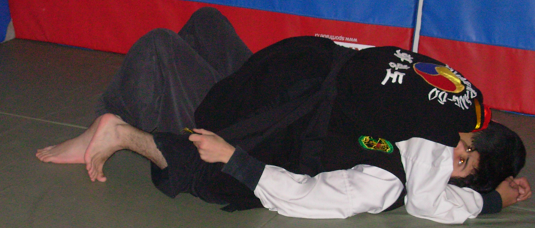
\includegraphics[width=0.5\textwidth]{images/Lucha_de_Piso/12_inmovilizacion_montado.png}
		\caption{Inmovilización de montada}
		\label{fig:posicion_montada}
	\end{figure}

	\item \textbf{Inmovilización de tijeras:}     La "Posición de Tijeras" es una técnica en HwaRangDo en la cual el ejecutor utiliza sus piernas para abrazar al oponente. Ver \ref{fig:posicion_tijeras}.

	En esta posición:

	\begin{itemize}
		\item El practicante entrelaza sus piernas alrededor del cuerpo del oponente.
		\item Esta técnica crea un bloqueo efectivo y limita la capacidad de movimiento del oponente.
		\item La "Posición de Tijeras" puede ser utilizada como una estrategia de control en el suelo o como preparación para aplicar sumisiones adicionales.
	\end{itemize}

	La ''Posición de Tijeras`` es una herramienta importante en el arsenal de técnicas de control y sumisión de HwaRangDo, permitiendo al practicante mantener a raya al oponente y buscar oportunidades para asegurar la victoria. \footnote{Para obtener la victoria, el que abraza con las piernas, debe estar sobre la espalda del oponente sin estrangularlo} . Ver \ref{fig:posicion_tijeras}.

	\begin{figure}[h]
		\centering
		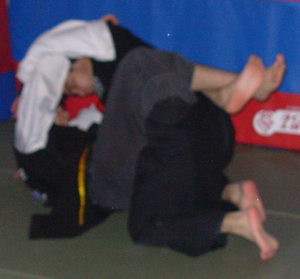
\includegraphics[width=0.5\textwidth]{images/Lucha_de_Piso/13_inmovilizacion_tijeras.png}
		\caption{Inmovilización de Tijeras}
		\label{fig:posicion_tijeras}
	\end{figure}
\end{enumerate}


\subsection{Técnicas avanzadas de inmovilización}

\begin{enumerate}

	\item \textbf{Inmovilización de tronco:} Explicación posición de Inmovilización de tronco. Ver \ref{fig:inmovilizacion_tronco_1}. Ver \ref{fig:inmovilizacion_tronco_2}.

	\begin{figure}[h]
		\centering
		\begin{minipage}{0.45\textwidth}
			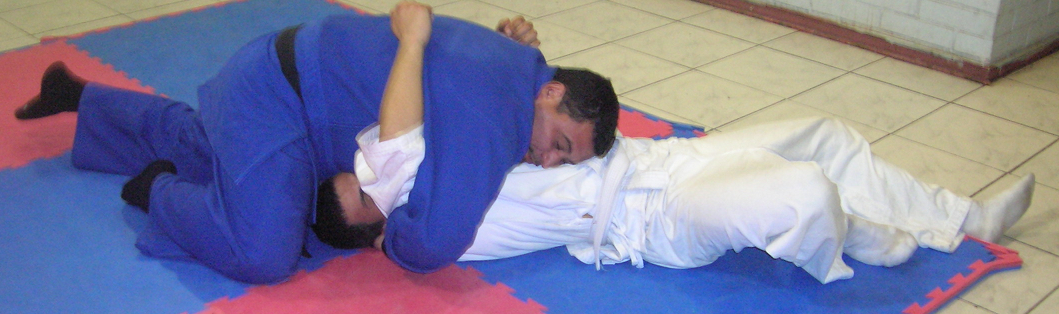
\includegraphics[width=\linewidth]{images/Lucha_de_Piso/14_inmovilizacion_pecho.png}
			\caption{Posición de retención lateral vista frontal}
			\label{fig:inmovilizacion_tronco_1}
		\end{minipage}
		\hfill
		\begin{minipage}{0.45\textwidth}
			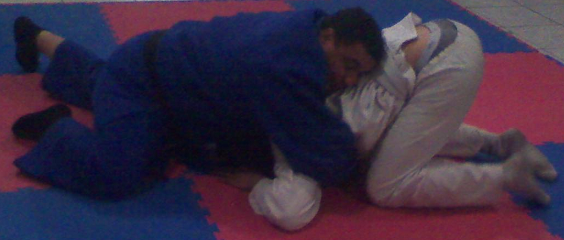
\includegraphics[width=\linewidth]{images/Lucha_de_Piso/15_inmovilizacion_pecho.png}
			\caption{Inmovilización lateral vista lateral}
			\label{fig:inmovilizacion_tronco_2}
		\end{minipage}
		\hfill
	\end{figure}


	\begin{figure}[h]
		\centering
		\begin{minipage}{0.45\textwidth}
			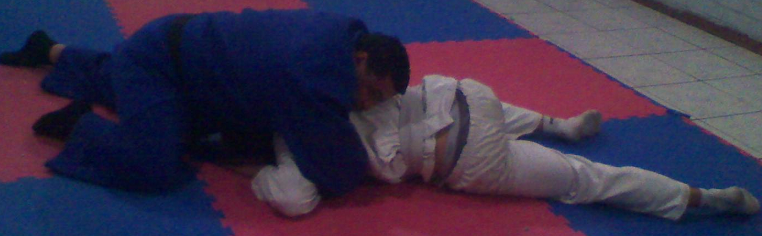
\includegraphics[width=\linewidth]{images/Lucha_de_Piso/16_inmovilizacion_pecho.png}
			\caption{Posición de retención lateral vista frontal}
			\label{fig:inmovilizacion_tronco_3}
		\end{minipage}
		\hfill
		\begin{minipage}{0.45\textwidth}
			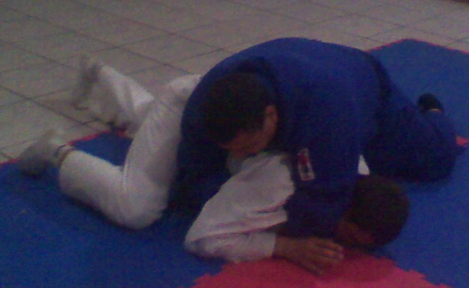
\includegraphics[width=\linewidth]{images/Lucha_de_Piso/17_inmovilizacion_pecho.png}
			\caption{Inmovilización lateral vista lateral}
			\label{fig:inmovilizacion_tronco_4}
		\end{minipage}
		\hfill
	\end{figure}


	\item \textbf{Inmovilización de Pulpo con tomada de brazo:} Explicación posición de Inmovilización de tronco. Ver \ref{fig:inmovilizacion_tronco_1}. Ver \ref{fig:inmovilizacion_tronco_2}.
	\begin{figure}[h]
		\centering
		\begin{minipage}{0.45\textwidth}
			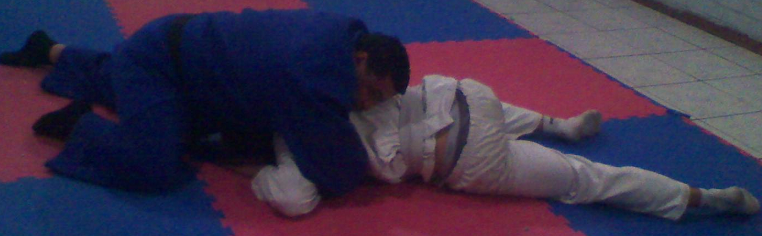
\includegraphics[width=\linewidth]{images/Lucha_de_Piso/16_inmovilizacion_pecho.png}
			\caption{Posición de retención lateral vista frontal}
			\label{fig:inmovilizacion_pulpo_arriba_tomada_de brazo}
		\end{minipage}
		\hfill
	\end{figure}

	\item \textbf{Inmovilización de Pulpo con tomada de brazo doble:} Explicación posición de Inmovilización de tronco. Ver \ref{fig:inmovilizacion_tronco_1}. Ver \ref{fig:inmovilizacion_tronco_2}.
	\begin{figure}[h]
		\centering
		\begin{minipage}{0.45\textwidth}
			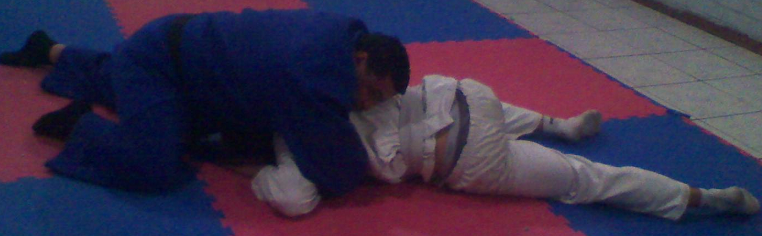
\includegraphics[width=\linewidth]{images/Lucha_de_Piso/16_inmovilizacion_pecho.png}
			\caption{Posición de retención lateral vista frontal}
			\label{fig:inmovilizacion_pulpo_arriba_tomada_de brazo_doble}
		\end{minipage}
		\hfill
	\end{figure}

	\item \textbf{Inmovilización de espalda:} Explicación posición de Inmovilización de tronco. Ver \ref{fig:inmovilizacion_tronco_1}. Ver \ref{fig:inmovilizacion_de_espalda}.
	\begin{figure}[h]
		\centering
		\begin{minipage}{0.45\textwidth}
			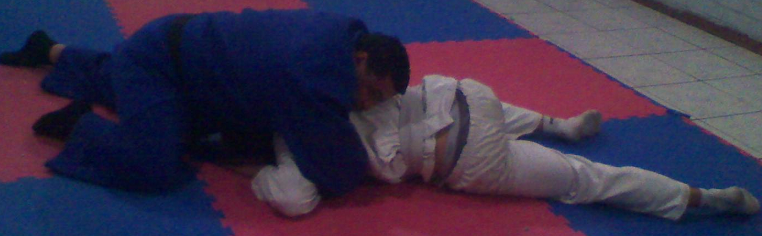
\includegraphics[width=\linewidth]{images/Lucha_de_Piso/16_inmovilizacion_pecho.png}
			\caption{Posición de retención de espalda}
			\label{fig:inmovilizacion_de_espalda}
		\end{minipage}
		\hfill
	\end{figure}

\end{enumerate}

%	\include{faja_celeste_amarillo}
%	\include{faja_amarilla}
%	\include{faja_amarilla_verde}
%	\include{faja_verde}
%	\include{faja_verde_azul}
%	\include{faja_azul}

%	\section{Bibliografía}

Aquí se menciona la página web sobre Hwarangdo\textregistered \cite{pagina-web}.

\bibliographystyle{apacite}
\bibliography{bibliografia}

	% Sección del glosario

	\include{glosario}
	\chapter{Glosario}
	\addcontentsline{toc}{chapter}{Glosario} % Agregar la sección al índice
	\printglossaries

	\appendix

	\clearpage

	\printglossary

	\clearpage

	\appendix

	\section{Anexo A: Alfabeto coreano y su romanización}

Este anexo contiene información adicional sobre el alfabeto coreano y su romanización.

\subsection{Historia del hangul}

El hangul fue creado en 1443 por el rey Sejong el Grande de Corea. El rey Sejong quería crear un sistema de escritura que fuera fácil de aprender y usar para todos los coreanos, independientemente de su nivel de educación o estatus social.

\subsection{Diferentes sistemas de romanización}

Además del sistema McCune-Reischauer, hay otros sistemas de romanización del hangul, como el sistema Yale y el sistema Revised Romanization of Korean (RR).

La siguiente tabla muestra la transliteración de las letras del hangul al sistema McCune-Reischauer:


\begin{table}[t]
	\caption{Romanización McCune-Reischauer}
	\begin{center}
		\begin{tabular}{ | m{2cm} | m{5cm} | m{5cm} | }
			\hline Hangul & McCune-Reischauer \\ \hline
			ㄱ & g \\
			ㄴ & n \\
			ㄷ & d \\
			ㄹ & r \\
			ㅁ & m \\
			ㅂ & b \\
			ㅅ & s \\
			ㅇ & ng \\
			ㅈ & j \\
			ㅊ & ch \\
			ㅋ & k \\
			ㅌ & t \\
			ㅍ & p \\
			ㅎ & h \\
			ㅏ & a \\
			ㅑ & ya \\
			ㅓ & o \\
			ㅕ & yo \\
			ㅗ & o \\
			ㅛ & yo \\
			ㅜ & u \\
			ㅠ & yu \\
			ㅡ & eu \\
			ㅣ & i \\ \hline
		\end{tabular}
	\end{center}
\end{table}



























\subsection{Ejemplos de uso del hangul}

A continuación se muestran algunos ejemplos de cómo se utiliza el hangul en la escritura coreana:

* El nombre del país Corea del Sur se escribe en hangul como 대한민국 (Daehanminguk).
* El nombre de la ciudad de Seúl se escribe en hangul como 서울 (Seoul).
* El nombre de la persona Kim Jong-un se escribe en hangul como 김정은 (Kim Jeong-un).


\end{document}